\chapter{Conclusion \& Future Work}

\section{Conclusion}

In this project, we have established a robust foundation for developing an accurate pose detection system tailored to classical performing arts, with a focus on Kathakali. Through a structured approach, we collected a diverse set of high-quality images, curated them carefully, and executed detailed annotations to capture the nuances of traditional poses and gestures. The annotated dataset, enriched with both bounding boxes and landmarks for key body points, forms a valuable resource for training specialized object detection models. This dataset not only supports the precise recognition of poses but also addresses the unique challenges of traditional attire and complex body movements inherent to the art form. By focusing on culturally significant gestures and postures, this system aims to contribute to both the preservation of heritage and advancements in pose detection technologies.
\section{Future Work}

In the next phase of our project, we will integrate state-of-the-art models for object detection and human landmarking to build a robust pose detection system. Our approach will involve selecting a suitable object detection model for initial body detection, followed by advanced landmark detection models tailored to capture the detailed and culturally specific poses of classical dance. Here’s an overview of potential models and their trade-offs:

Object Detection Models
For the task of detecting performers and creating bounding boxes around them, we will explore high-performance object detection models known for their accuracy and speed:

\begin{itemize}
    \item YOLOv5
    \begin{itemize}
            \item Pros: Known for its speed and accuracy, especially suitable for real-time applications; performs well on resource-constrained devices.
    \item Cons: Requires substantial training data to generalize well; may struggle with finer details when the subject is wearing intricate costumes typical in traditional performances.
    \end{itemize}
    \item Faster R-CNN
    \begin{itemize}
            \item Pros: Delivers high accuracy, particularly in detecting complex scenes; suitable for high-resolution images.
    \item Cons: Computationally intensive; slower than YOLO models, making it less suitable for real-time applications with video input.
    \end{itemize} 

    \item EfficientDet
        \begin{itemize}
            
    \item Pros: Optimized for a balance between accuracy and efficiency; scalable for different device capabilities.
    \item Cons: Moderate accuracy compared to YOLO and Faster R-CNN, especially when dealing with densely packed or intricate object features.
        \end{itemize}
\end{itemize}
The choice of object detection model will depend on the system requirements and available computational resources. YOLOv5, with its speed and accuracy, may be a suitable choice for the first iteration of our system.

Human Landmarking Models
Once the body is detected, the next step involves recognizing key body landmarks that define the pose. We’ll assess the following models, each with unique advantages for detailed human landmark detection in complex poses:

\begin{itemize}
    \item HRNetv2/HigherHRNet
    \begin{itemize}
        \item Pros: Known for exceptional accuracy in multi-person pose estimation; effective at capturing fine details and handling complex body postures, which is valuable for classical dance poses.
    \item Cons: High computational cost, making it slower for real-time processing; requires more powerful GPUs to perform effectively in video-based applications.
    \end{itemize}
    \item OpenPose
    \begin{itemize}
        \item Pros: Well-established for multi-person and full-body pose detection; accurate in detecting body, face, and hand landmarks.
    \item Cons: Computationally intensive, especially for video inputs; may not perform as effectively on mobile devices or low-power systems.
    \end{itemize}
    
    \item Convolutional Pose Machines
    \begin{itemize}
            \item Pros: Modular and interpretable, with an ability to handle challenging poses by stacking multiple stages of pose refinement; offers strong accuracy for detailed landmark detection.
    \item Cons: Relatively slower compared to more recent models like HRNet; less optimized for real-time applications, which could limit scalability.
    \end{itemize}    

    \item PoseNet
    \begin{itemize}
            \item Pros: Lightweight and efficient, capable of running on mobile and web platforms; suitable for applications that prioritize speed over extreme accuracy.
    \item Cons: Limited accuracy compared to HRNet and OpenPose, especially for detailed and culturally specific poses that involve complex gestures.
    \end{itemize}
\end{itemize}

The selected object and pose detection models will be trained and optimized using our curated dataset. The system’s workflow will proceed as follows:

\begin{enumerate}
    \item Input Layer: Receives video or image files as input.
    \item Preprocessing Layer: Filters out background noise, enhancing the clarity of the input data.
    \item Body Detection Module: Uses the chosen object detection model (e.g., YOLOv5) to locate the performer within the frame.
    \item Landmark Detection Module: Applies the selected landmark detection model (e.g., HRNetv2) to mark essential body points, including joints, head, limbs, etc.
    \item Output Layer: Provides processed frames with detailed pose annotations, ready for further analysis.
\end{enumerate}
This integrated pipeline will enable us to achieve precise pose detection tailored to traditional performing arts, offering a valuable tool for cultural preservation and contributing to advancements in pose detection within underrepresented contexts.

\begin{figure}[h]
\centering
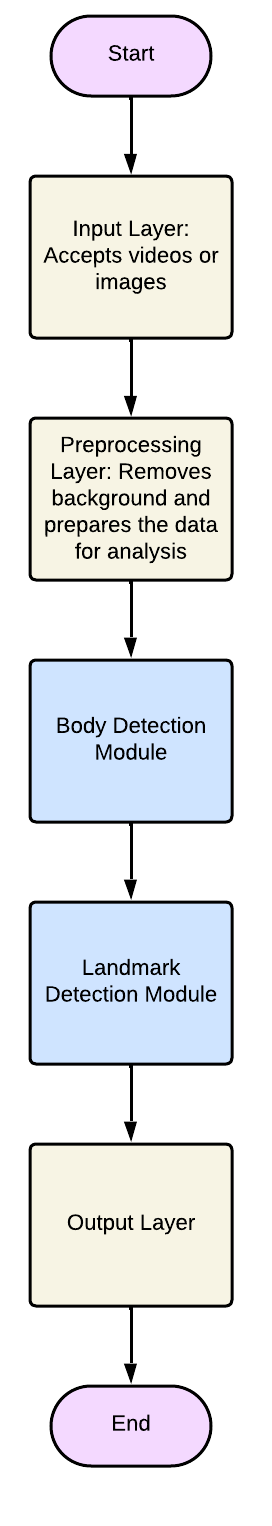
\includegraphics[width=0.24\linewidth]{image1.png}
\caption{System workflow for the proposed system.}
\end{figure}


